\RequirePackage{fix-cm}
%
\RequirePackage{amsmath}

%\documentclass{svjour3}                     % onecolumn (standard format)
%\documentclass[smallcondensed]{svjour3}     % onecolumn (ditto)
%\documentclass[smallextended]{svjour3}       % onecolumn (second format)
\documentclass[twocolumn]{svjour3}          % twocolumn
%\documentclass[letterpaper, 12pt, twocolumn]{article}

%\usepackage[margin=1in]{geometry}
\usepackage{amssymb}
\usepackage{graphicx}
\usepackage[utf8]{inputenc}
\usepackage{indentfirst}
%\usepackage{physics}
\newcommand{\me}{\mathrm{e}}
\usepackage{amsmath}

%\usepackage[round]{natbib}
%\usepackage{apacite}
\usepackage{url}

% For the flow charts
\usepackage{tikz}
\usetikzlibrary{shapes.geometric, arrows, calc, positioning}
\tikzstyle{startstop} = [rectangle, thick, rounded corners=2.5mm, minimum width=2cm, minimum height=5mm,text centered, draw=black]
\tikzstyle{io} = [trapezium, thick, trapezium left angle=70, trapezium right angle=110, text width=3.75cm, minimum height=0.5cm, text centered, draw=black]
\tikzstyle{process} = [rectangle, thick, minimum width=2.5cm, text width=4cm, minimum height=0.5cm, text centered, draw=black]
\tikzstyle{decision} = [diamond, thick, minimum width=3cm, minimum height=1cm, text centered, draw=black]
\tikzstyle{dottedbox} = [rectangle, dotted, thick, minimum width=2.5cm, text width=2.8cm, minimum height=0.5cm, text centered, draw=black]
\tikzstyle{arrow} = [thick,->,>=stealth]
\tikzstyle{dottedarrow} = [thick, dotted,->,>=stealth]



\usepackage{pgfplots}
\usepgfplotslibrary{patchplots}
\pgfplotsset{compat=newest, samples=065} %Set this value to 65 for the final version
%\usepgfplotslibrary{dateplot} 


%\providecommand{\keywords}[1]{\textbf{\textit{Index terms---}} #1}

\journalname{Journal of Science Education and Technology}

\begin{document}
	
	
	\title{Algorithm to generate multi-factorial experiments to teach experimental design%\thanks{Grants or other notes
		%about the article that should go on the front page should be
		%placed here. General acknowledgments should be placed at the end of the article.}
	}
	%\subtitle{Do you have a subtitle?\\ If so, write it here}
	%\titlerunning{Short form of title}        % if too long for running head
	\author{A.C.~Delgado-Chavez  \and
		N.~Balagurusamy \and
		R.~Narayanasamy \and
		S.~K.~Gadi
	}
	%\authorrunning{Short form of author list} % if too long for running head
	\institute{     \textbf{Ana Cristina Delgado-Chavez,} \\ \textbf{Nagamani Balagurusamy} \at
		Laboratorio de Biorremediación, Facultad de Ciencias Biológicas, Universidad Autónoma de Coahuila, Carretera Torreón-Matamoros Km 7.5, Torreón, Coahuila, México.
		\and
		\textbf{Rajeswari Narayanasamy} \at
		Facultad de Ingeniería, Ciencias y Arquitectura de la Universidad Juárez del Estado de Durango, Gomez Palacio, Durango. Mexico
		\and
		\textbf{S. K. Gadi} \at
		Facultad de Ingeniería Mecánica y Eléctrica, Universidad Autónoma de Coahuila, Carretera Torreón-Matamoros Km 7.5, Torreón, Coahuila, México.\\
		Tel.: (+52 1) 871 757 0239\\
		Fax: (+52 1) 871 757 0239\\
		\email{research@skgadi.com}
	}
	\date{Received: date / Accepted: date}
	% The correct dates will be entered by the editor
	\maketitle
	\begin{abstract}
		One of the challenges in teaching the subject, Design of Experiments, is to come up with a proper numerical example. In this article, authors present a methodology to generate a numerical example for multifactorial experiments. Also, it presents a simple algorithm, which can be implemented in any programming language to generate unique examples.
	\end{abstract}
	\keywords{Experimental design; educational tool; generating examples}
	\section{Introduction}
	Experimental design is applied in almost all the fields involving experimentation \cite{fisher1937design,quinn2002experimental,montgomery2008design,antony2014design}. It is part of various undergraduate and graduate curriculum, ranging from the engineering to the biological sciences. In general, the objective of experimental design is to minimize cost and time of the experiments and maximize the yield. As an example, in some cases with a lot of data to process, use of experimental designs help to find the optimal conditions for a process or in order to obtain the maximum yield of a product in a minimum number of experiments \cite{B703690F}. On the other hand, an improper design of experiment may lead to inaccurate or false conclusions, as well as a loss of money, material and time \cite{Festing2003341}.
	\par
	Learning statistics or mathematics in general is effective by solving a number of numerical examples \cite{zhu1987learning}. It helps the students to develop insight in the topics \cite{renkl1997learning}. It is well documented that students show good learning experience using visual examples and perform better with the examples of experiments which they can relate \cite{hattie2013visible}. Teachers may involve students in finding experiments to teach the topic \cite{Hunter1977Some,fried2006mathematics,Hiebert82}. However, it is teacher's task to generate examples for the classroom and for the practice \cite{Deborah2008}.
	\par
	Solving optimization problems and finding the most accurate mathematical model for a process/system in experimental design involves performing various experiments with different combinations of the factors. Conducting experiments on a real system for the classroom purpose is not always feasible due to any of the following limitations.
	\begin{enumerate}
		\item The cost of conducting experiments on a real system is not always negligible.
		\item A considerable amount of time may take for each experiment.
		\item The combination of factors associated for optimum response is constant for a physical system. Therefore, teachers may not provide a fresh problem.
	\end{enumerate}
	\par
	Hence, a computer program generating responses for the given input factors is a good alternative to mimic the physical systems. In this article a methodology is presented to generate numerical examples which simulate experiments. The objective is to generate unique process for the limits selected by the user, which outputs experimental data for the given combinations of the factors. Teachers may adopt this methodology in generating numerical examples, which highlight all the characteristics they want to present to the classroom, give as practice exercise and conduct exams.
	\par
	The proposed algorithm is described in Section \ref{Sec:Algorithm}. Readers interested only in the implementation of algorithm may skip the mathematical construction presented in Section \ref{Sec:Construction} and \ref{Sec:Adapting}.
	\par
	A numerical example for an experimental design is a mathematical model representing a physical process. This model is a set of static functions (i.e. it does not have derivative or integral terms) which maps the factors to the responses. A real life system may present more than one peaks. However, most of the experimental design methods find the local maximum based on the initial base value. Hence, the proposed algorithm is designed to present only one peak. A multi-response system can be represented as %Because time is also a factor
	\begin{eqnarray}
	y_j &=& f_j(x_1, x_2, x_3, \dots, x_n) + \xi_j \label{Eqn:Function}
	\end{eqnarray}
	\noindent where $y_j$, $j\in \{1,2,3, \dots, m\}$ are the responses, $x_i$, $i\in \{1,2,3, \dots, n\}$ are the factors, $f_j$, $j\in \{1,2,3, \dots, m\}$ are the nonlinear functions mapping the $n$ factors to the $m$ responses and $\xi_i$, $i\in \{1,2,3, \dots, m\}$ are the noise.
	\par
	All the factors, $x_i$, are constrained by upper and lower limits. The numerical examples should produce a unique optimal responses, $y_j^M$, for a set of factors within its limits. Construction of a one such mathematical function is presented in the next section.
	\par
	The proposed algorithm presents the case of single response, which can be adopted to multi-response.
	\section{Construction of a mathematical function to suit our requirements}
	\label{Sec:Construction}
	In this section possible candidates for the function $f_i$  are discussed. The selected candidate function is then adapted to meet our further requirements in the next section.
	\subsection{Quadratic concave function}
	\begin{figure}
		\centering
		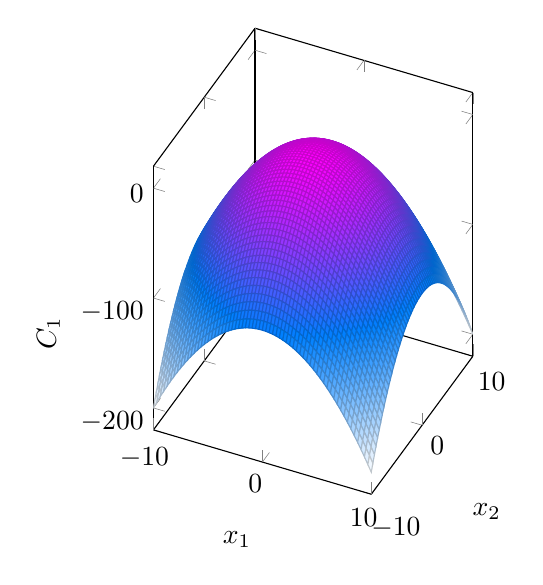
\begin{tikzpicture}
		\begin{axis}[
		width=0.465\textwidth,	
		height = 7.5cm,
		colormap/cool,
		xlabel=$x_1$,
		ylabel=$x_2$,
		zlabel=$C_1$,
		]
		\addplot3[
		surf,
		%samples=10,
		domain=-10:10,
		]
		{-x^2-y^2};
		%\addlegendentry{$\frac{sin(r)}{r}$}
		\end{axis}
		\end{tikzpicture}
		\caption{Quadratic concave function $C_1(x_1, x_2)$.}
		\label{Fig:TwoVariablePolynomial}
	\end{figure}
	A second order polynomial function, such as
	\begin{eqnarray}
	C_1(x_1, x_2, x_3, \dots, x_n) &:=& -\sum_{i=1}^{n}{x_i^2} \label{Eqn:PolyFunction}
	\end{eqnarray}
	is a concave function, which serve the purpose of providing a unique optimal point. Fig.~\ref{Fig:TwoVariablePolynomial} depicts (\ref{Eqn:PolyFunction}) for the two variables case. However, it doesn't meet the requirements of a good example because to the following limitations.
	\begin{enumerate}
		\item Response surface methodology uses a second order fit algorithm. Hence, the process of reaching optimal solution becomes trivial.
		\item A quadratic function is having a property that its slope increases as it moves far from the optimal point. This property trivializes the process of selecting a new base value.
	\end{enumerate}
	\subsection{Multivariable Gaussian function}
	\begin{figure}
		\centering
		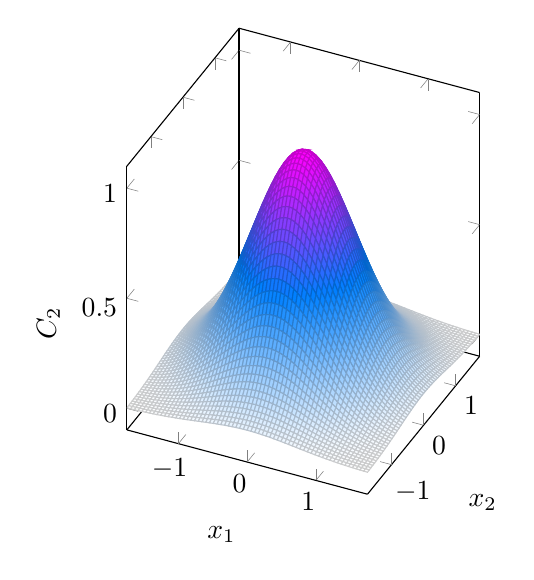
\begin{tikzpicture}
		\begin{axis}[
		width=0.50\textwidth,	
		height = 7.5cm,
		colormap/cool,
		xlabel=$x_1$,
		ylabel=$x_2$,
		zlabel=$C_2$,
		]
		\addplot3[
		surf,
		%samples = 10,
		domain=-1.75:1.75,
		]
		{exp(-x^2-y^2)};
		\end{axis}
		\end{tikzpicture}
		\caption{Two variable Gaussian function $C_2(x_1, x_2)$.}
		\label{Fig:TwoVarGaussian}
	\end{figure}
	The multivariable Gussian function
	\begin{eqnarray}
	C_2(x_1, x_2, x_3, \dots, x_n) := \prod_{i=1}^{n}{\me^{-x_i^2}} \label{Eqn:MultiFactorialNormal}
	\end{eqnarray}
	is a concave function, hence, it has a unique maximum value. The slope of this function is not linearly related with the distance from its optimal point. The concave functions have property that the response of all the points between any two arbitrary points always grater than the responses at these arbitrary points \cite{antoniou2007practical}. A non-concave function gives additional challenge in solving the optimization problem. 
	\subsection{Modified version of Gaussian function}
	\begin{figure}
		\centering
		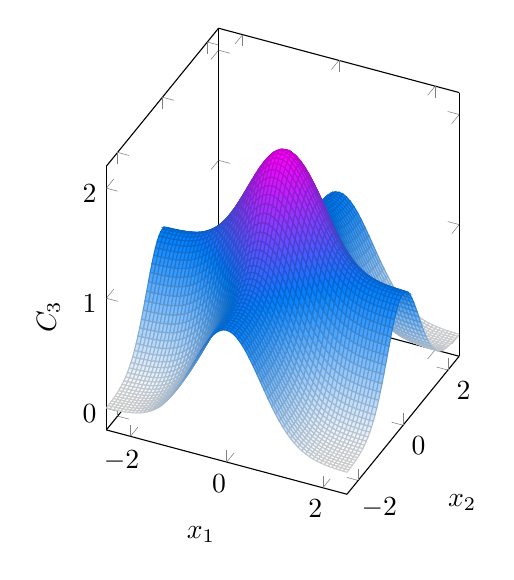
\begin{tikzpicture}
		\begin{axis}[
		width=0.50\textwidth,	
		height = 7.5cm,
		colormap/cool,
		xlabel=$x_1$,
		ylabel=$x_2$,
		zlabel=$C_3$,
		]
		\addplot3[
		surf,
		%samples = 50,
		domain=-2.5:2.5,
		]
		{exp(-x^2)+exp(-y^2)};
		\end{axis}
		\end{tikzpicture}	
		\caption{Modified version of Gaussian function $C_3(x_1, x_2)$.}
		\label{Fig:2GussianFunctionModified}
	\end{figure}
	
	
	
	
	Keeping above limitations in mind, a modified version of Gussian function is proposed as
	\begin{eqnarray}
	C_3(x_1, x_2, x_3, ..., x_n) := \sum_{i=1}^{n}{\me^{-x_i^2}}. \label{Eqn:ModifiedGuassian}
	\end{eqnarray}
	\par
	Fig.~\ref{Fig:2GussianFunctionModified} depicts (\ref{Eqn:ModifiedGuassian}) for the case of two variables. A symmetric matrix is called negative definite when all its eigenvalues are negative. A function can be said concave, if Hessian matrix associated with it is negative definite \cite{bernstein1962some}. Hessian matrix for (\ref{Eqn:ModifiedGuassian}) is 
	\begin{eqnarray}
	H_{i,j} = \frac{\partial^2 C_3}{{\partial x_i}^2} =
	\begin{cases}
	2\me^{-x_i^2}(2x_i^2-1)	,	& \text{if } i = j\\
	0						,	& \text{otherwise}
	\end{cases} \label{Eqn:HessianMatrix}
	\end{eqnarray}
	where $i, j \in \{1, 2, 3, \dots, n\}$.
	\par
	The above equation shows that the Hessian matrix, $H$, is a diagonal matrix. In a diagonal matrix each element on the principal diagonal is an eigenvalue. So, it can be said that this matrix is not a negative definite because there exist positive elements for $|x_i|>\sqrt{\frac{1}{2}}$.
	\par
	In a function gradient is zero at the peaks, dips and saddle points. The gradient vector of (\ref{Eqn:ModifiedGuassian}) is
	\begin{eqnarray}
	\Delta C_{3_i} = \frac{\partial C_3}{\partial x_i} = -2x_i\me^{-x_i^2} \label{Eqn:GradientModifiedGuassian}
	\end{eqnarray}
	where $i \in \{1, 2, 3, \dots, n\}$. $\Delta C_{3_i} = 0$ implies $x_i =0$ or $x_i=\pm\infty$. Hence, it is guaranteed that there exists only one peak at $x_1 = x_2 = x_3 = \dots = x_n = 0$.
	\par
	In this function, the optimum value for any $i^{\text{th}}$ factor is unaffected with the other factors. This is not recommended because it trivializes the multi-factorial problems.
	\subsection{A novel mathematical function}
	\begin{figure}
		\centering
		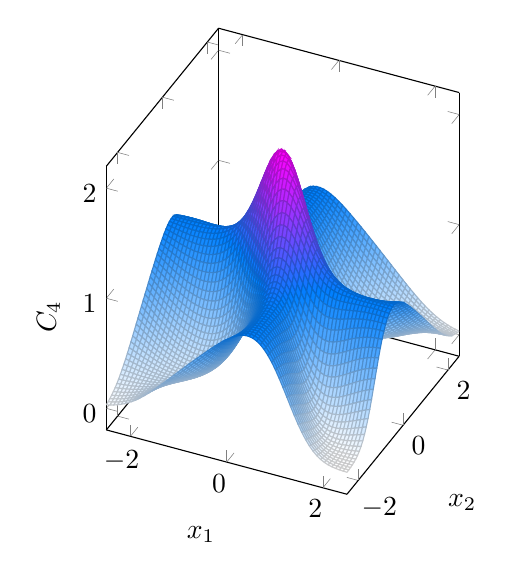
\begin{tikzpicture}
		\begin{axis}[
		width=0.50\textwidth,	
		height = 7.5cm,
		colormap/cool,
		xlabel=$x_1$,
		ylabel=$x_2$,
		zlabel=$C_4$,
		]
		\addplot3[
		surf,
		%samples = 50,
		domain=-2.5:2.5,
		]
		{exp(-(x+0.49*sin(deg(x+y)))^2)+exp(-(y+0.49*sin(deg(x+y)))^2)};
		\end{axis}
		\end{tikzpicture}
		\caption{The proposed function $C_4(x_1, x_2)$ for $a = 0.49$.}
		\label{Fig:TwoVarNovelFunc}
	\end{figure}
	The following mathematical function is proposed by introducing a new nonlinear term to the above model.
	\begin{eqnarray}
	C_4(.) := \sum_{i=1}^{n}{\exp[-\left(x_i + a\sin\left(\sum_{i=1}^{n} x_i\right)\right)^2]} \label{Eqn:Novelmodel}
	\end{eqnarray}
	\par
	Fig.~\ref{Fig:TwoVarNovelFunc} depicts $C_4$ for a two variable case with $a=0.49$. The gradient of $C_4$ is
	\begin{eqnarray}
	\Delta C_{4_i} &=& \frac{\partial C_4}{\partial x_i} \nonumber\\
	&=& -2\exp[-\left(x_i + a\sin\left(\sum_{i=1}^{n} x_i\right)\right)^2] \times \nonumber\\
	&& \left[ x_i + a\sin\left(\sum_{i=1}^{n} x_i\right) \right] \left[1 + a\cos\left(\sum_{i=1}^{n} x_i\right) \right] \label{Eqn:GradientNovelFunc}
	\end{eqnarray}
	where $i \in \{1, 2, 3, \dots, n\}$. Peaks, dips or saddle points form at 
	\begin{eqnarray}
	\Delta C_{4_i}=0 \label{Eqn:GradientNovelEqn}
	\end{eqnarray}
	Only one peak is required, other peaks, dips and saddle points should be suppressed. Equation (\ref{Eqn:GradientNovelEqn}) can be solved by solving the following three equations.
	\begin{eqnarray}
	\exp[-\left(x_i + a\sin\left(\sum_{i=1}^{n} x_i\right)\right)^2]=0 \label{Eqn:GradientNovelEqn1} \\
	x_i + a\sin\left(\sum_{i=1}^{n} x_i\right)=0 \label{Eqn:GradientNovelSol2} \\
	1 + a\cos\left(\sum_{i=1}^{n} x_i\right)=0 \label{Eqn:GradientNovelEqn3}
	\end{eqnarray}
	The solution for (\ref{Eqn:GradientNovelEqn1}) is $|x_i|=\infty$, which can be ignored. The solution for (\ref{Eqn:GradientNovelEqn3}) is
	\begin{eqnarray}
	\sum_{i=1}^{n} x_i &=& \cos[-1](\frac{-1}{a}) \label{Eqn:GradientNovelSol3}
	\end{eqnarray}
	Selecting a value $|a|<1$, all the real solutions of (\ref{Eqn:GradientNovelSol3})  can be suppressed. Equation (\ref{Eqn:GradientNovelSol2}) can be rewritten as 
	\begin{eqnarray}
	x_i = -a\sin\left(\sum_{i=1}^{n} x_i\right) \label{Eqn:GradientNovelSol2ReWr1}
	\end{eqnarray}
	which implies that the solution lies at $x_1 = x_2 = x_3 = \dots = x_n$. Hence (\ref{Eqn:GradientNovelSol2ReWr1}) can be rewritten it as
	\begin{eqnarray}
	nx_i + na\sin(nx_i) = 0 \label{Eqn:GradientNovelSol2ReWr2}
	\end{eqnarray}
	Since $|\sin(p)|<p$ for all the values of $p$ except for $p = 0$, the solution can be limited to only one point $x_1 = x_2 = x_3 = \dots = x_n=0$ provided that $|na|<1$. Considering a positive value for $a$, only one peak at origin for $a<\frac{1}{n}$ is  guaranteed.
	\par
	In the next section a method is presented to adapt the function $C_4$ defined at (\ref{Eqn:Novelmodel}) to generate random experiments.
	\section{Adapting the proposed function}
	\label{Sec:Adapting}
	Noise is added.
	A scaled version of the function $C_4$ proposed in (\ref{Eqn:Novelmodel}) is
	\begin{eqnarray}
	f&&(x_1, x_2, x_3, \dots, x_n) = \nonumber \\
	F&&(z_1, z_2, z_3, \dots, z_n) := F_1 +  \nonumber \\
	&& \frac{F_2}{n}\left[\sum_{i=1}^{n}{\exp[-\left[z_i + a\sin\left(\Sigma_z\right)\right]^2]} + K_R\xi\right], \label{Eqn:AdaptedFunction}
	\end{eqnarray}
	\begin{eqnarray}
	F_1 &:=& F_L+\alpha F_I\Xi, \label{Eqn:F_1Equation} \\
	F_2 &:=& (1-2\alpha)F_I\Xi, \label{Eqn:F_2Equation} \\
	F_I &:=& (F_U-F_L), \label{Eqn:FunctionInterval} \\
	\Xi &:=& 0.5 (\xi + 1), \label{Eqn:ChangeOfRandomVar} \\
	\Sigma_z &:=& \sum_{i=1}^{n} z_i, \label{Eqn:SigmaZ} \\
	z_i &:=& \frac{K_D(x_i-x_i^M)}{x_i^I}, \label{Eqn:ZiDefinition} \\
	x_i^I &:=& x_i^U - x_i^L, \label{Eqn:InterDefinition} \\
	x_i^M &:=& x_i^L + \beta x_i^I+(1-2\beta)x_i^I\Xi, \label{Eqn:FactorAtMaximumValue}
	\end{eqnarray}
	\begin{eqnarray}
	0 < \alpha < 0.5, \label{Eqn:ConstraintsForAlpha} \\
	0 < \beta < 0.5, \label{Eqn:ConstraintsForBeta}
	\end{eqnarray}
	where  $i \in \{1, 2, 3, \dots, n\}$, $\xi$ is a random variable with the properties $E(\xi)=0$ and $|\xi|\le 1$, $\Xi$ is a random variable with the properties $E(\Xi)=0.5$ and $0 \le \xi \le 1$,  $E(.)$ is the expected value. $[F_L, F_U]$ is the function range, $K_R$ is a noise factor, $K_D$ is difficulty factor, $x_i^M$ are the optimal combination of factors where the function $g$ reaches its maximum value, $x_i^L$ and $x_i^U$ are lower and upper limit of the $i^{\text{th}}$ factor, $\alpha$ and $\beta$ are padding constants for limiting the maximum value of the function $f$ and limiting the optimal combination within the desired region respectively.
	\par
	The function $F(z_1, z_2, z_3, \dots, z_n)$ of (\ref{Eqn:AdaptedFunction}) preserves all the following mathematical properties of the function $C_4$ proposed in (\ref{Eqn:Novelmodel}).
	\begin{enumerate}
		\item Gradient is not proportional to the distance from its optimum combination.
		\item Has unique maximum value at $z_1 = z_2 = z_3 = \dots = z_n = 0$ i.e. at $x_i=x_i^M, \forall i\in\{1, 2, 3, \dots, n\}$, provided that $a<\frac{1}{n}$
		\item It is not a concave function.
		\item The optimal value of an arbitrary factor is not constant throughout the factorial space.
	\end{enumerate}
	\par
	In the next section, an algorithm is presented to show implementation procedure.
	\section{Algorithm}
	\label{Sec:Algorithm}
	\begin{figure}
		\centering
		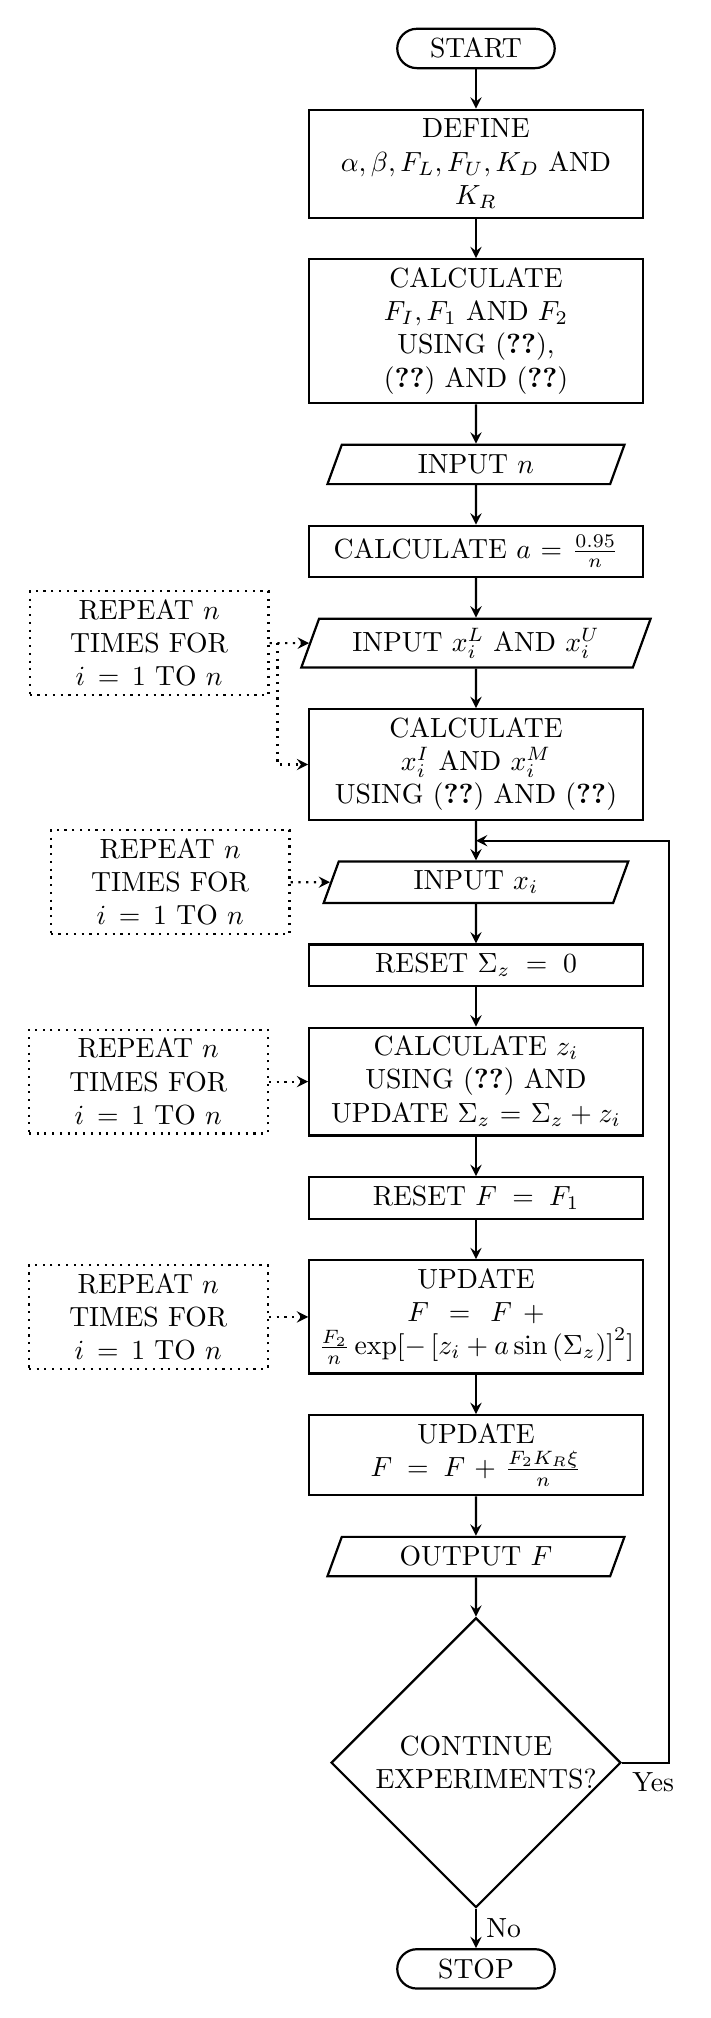
\begin{tikzpicture}[node distance = 5mm, auto]
		\node (Start) [startstop] {START};
		\node (Define) [process, below = of Start] {DEFINE $\alpha, \beta, F_L, F_U, K_D$~AND $K_R$};
		\node (Calculate01) [process, below =of Define] {CALCULATE\\$F_I, F_1$ AND $F_2$\\USING (\ref{Eqn:F_1Equation}), (\ref{Eqn:F_2Equation}) AND (\ref{Eqn:FunctionInterval})};
		\node (Input01) [io, below = of Calculate01, text width=3cm] {INPUT $n$};
		\node (Calculate01a) [process, below = of Input01] {CALCULATE $a=\frac{0.95}{n}$};
		\node (Input02) [io, below = of Calculate01a] {INPUT $x_i^L$~AND~$x_i^U$};
		\node (Calculate02) [process, below = of Input02] {CALCULATE\\$x_i^I$ AND $x_i^M$\\USING (\ref{Eqn:InterDefinition}) AND (\ref{Eqn:FactorAtMaximumValue})};
		\node (Input03) [io, below = of Calculate02, text width=3.25cm] {INPUT $x_i$};
		\node (Calculate03) [process, below = of Input03] {RESET $\Sigma_z=0$};
		\node (Calculate04) [process, below = of Calculate03] {CALCULATE $z_i$\\ USING (\ref{Eqn:ZiDefinition}) AND\\UPDATE $\Sigma_z = \Sigma_z + z_i$};
		\node (Calculate05) [process, below = of Calculate04] {RESET $F=F_1$};
		\node (Calculate06) [process, below = of Calculate05] {UPDATE\\  $F=F+\frac{F_2}{n} \exp[-\left[z_i + a\sin\left(\Sigma_z\right)\right]^2]$};
		\node (Calculate07) [process, below = of Calculate06] {UPDATE	\\ $F=F+\frac{F_2K_R\xi}{n}$};
		\node (Output03) [io, below = of Calculate07, text width=3cm] {OUTPUT $F$};
		\node (Decision01) [decision, below = of Output03, text width=2.55cm] {CONTINUE\\EXPERIMENTS?};
		\node (Stop) [startstop, below = of Decision01] {STOP};
		
		\node (ForBox01) [dottedbox, left = of Input02, left = 5mm] {REPEAT $n$ TIMES FOR $i=1$ TO $n$};
		%\node (ForBox02) [dottedbox, left of=Calculate02, left = 2.25cm] {REPEAT $n$ TIMES FOR $i=1$ TO $n$};
		\node (ForBox03) [dottedbox, left = of Input03, left = 5mm] {REPEAT $n$ TIMES FOR $i=1$ TO $n$};
		\node (ForBox04) [dottedbox, left = of Calculate04, left = 5mm] {REPEAT $n$ TIMES FOR $i=1$ TO $n$};
		\node (ForBox05) [dottedbox, left = of Calculate06, left = 5mm] {REPEAT $n$ TIMES FOR $i=1$ TO $n$};
		
		%\node (stop) [startstop, below of=calculate1, below = 0mm] {STOP};
		\draw [arrow] (Start) -- (Define);
		\draw [arrow] (Define) -- (Calculate01);
		\draw [arrow] (Calculate01) -- (Input01);
		\draw [arrow] (Input01) -- (Calculate01a);
		\draw [arrow] (Calculate01a) -- (Input02);
		\draw [arrow] (Input02) -- (Calculate02);
		\draw [arrow] (Calculate02) -- (Input03);
		\draw [arrow] (Input03) -- (Calculate03);
		\draw [arrow] (Calculate03) -- (Calculate04);
		\draw [arrow] (Calculate04) -- (Calculate05);
		\draw [arrow] (Calculate05) -- (Calculate06);
		\draw [arrow] (Calculate06) -- (Calculate07);
		\draw [arrow] (Calculate07) -- (Output03);
		\draw [arrow] (Output03) -- (Decision01);
		\draw [arrow] (Decision01) -- node[anchor=west]{No}(Stop);
		\draw [arrow] ($ (Decision01.east) $)node[anchor=north west]{Yes}  -- ++(0.6,0.00) |- ($ (Input03.north) + (0mm,2.5mm) $);
		
		\draw [dottedarrow] (ForBox01) -- (Input02);
		%\draw [dottedarrow] (ForBox02) -- (Calculate02);
		\draw [dottedarrow] ($(ForBox01.east) + (1mm,0mm)$) |- (Calculate02);
		\draw [dottedarrow] (ForBox03) -- (Input03);
		\draw [dottedarrow] (ForBox04) -- (Calculate04);
		\draw [dottedarrow] (ForBox05) -- (Calculate06);
		\end{tikzpicture}
		\caption{Flowchart of the proposed algorithm}
		\label{Fig:AlgorithmInFlowchart}
	\end{figure}
	Fig.~\ref{Fig:AlgorithmInFlowchart} shows the flowchart of the proposed algorithm. The values of $\alpha$ and $\beta$ should be less than 0.5. It is recommended to use $\alpha = \beta = 0.2$. $F_L$ and $F_U$ are lower and upper limits of the values generated in the experiments. Hence, user should select the values such that $F_L<F_U$. $K_D$ is the difficulty factor, the bigger the value is assigned, the harder it is to reach the optimum value. It is recommended to use a value $K_D=5$. The noise factor $K_R$ introduces noise into the system.
	\par
	Using the equations and inequalities given from (\ref{Eqn:AdaptedFunction}) to (\ref{Eqn:ConstraintsForBeta}), the algorithm generates responses for the given $x_i$ inputs.
	\section{Application}
	\label{Sec:Application}
	\begin{figure}
		\centering
		\begin{tikzpicture}
		\begin{axis}
		[
		width=0.50\textwidth,	
		view={0}{90}
		]
		\addplot3[contour gnuplot ={number=20,
			labels=false,
		},
		domain = 0:100,
		domain y = -1:1,
		%thick,
		]
		{193.0429025 + 137.9330151 *( exp(-(0.05 *(x-25.29101312) + 0.475*sin(deg(0.05 *(x-25.29101312) + 2.5* (y - 0.35586306))))^2) +
			exp(-(2.5* (y - 0.35586306) + 0.475*sin(deg(0.05 *(x-25.29101312) + 2.5 *(y - 0.35586306))))^2) )
		};
		\addplot3 [color= red,mark=*,] coordinates {
			(28.125, -0.4375, 320.3734872)
			(65.10367211, -0.562123929, 199.7015173)
			(46.82534862, -0.328866958, 262.9029596)
			(33.05522139, -0.038774837, 361.565507)
			(22.34726992, 0.299065229, 447.3591635)
			(25.01398522, 0.271862773, 455.5853246)
		};
		\end{axis}
		\end{tikzpicture}
		\caption{Contour plot of $F$ with the constants given in Section~$\ref{Sec:Application}$ superimposed with the RSM results.}
		\label{Fig:Application2Variable}
	\end{figure}
	The proposed algorithm shown in Fig.~\ref{Fig:AlgorithmInFlowchart} is implemented in the programing language JavaScript, which is complemented with a graphical user interface (GUI) designed in HTML and CSS. This application is used in the classroom for teaching Response Surface Methodology (RSM) to the master students of Biological Sciences Faculty, Universidad Autónoma de Coahuila, Torreón.
	\par
	This application is executed with $n=2$, $\alpha = \beta = 0.2$, $F_L = 100$, $F_U=600$, $K_D = 5$, $K_R = 0.1$, $x_1^L=0$, $x_1^U=100$, $x_2^L=-1$, and $x_2^U=1$. The application calculated $a= 0.475$, $F_1 = 193.043$, $F_2= 275.866$, $x_1^I=100$, $x_2^I=2$, $x_1^M=25.291$, and $x_2^M=0.356$. Fig.~\ref{Fig:Application2Variable} shows the contour plot of the function $f(x_1,x_2)$ generated with these constants. The RSM is applied to find the optimal values of $x_1$ and $x_2$, results of each iteration are also superimposed over the contours.
	%\cite{Multifac29:online}.
	\section{Conclusion}
	\label{Sec:Conclusion}
	The Construction of a single response, unique peak multivariable mathematical function for is presented. Later it is adapted to generate experimental data for a selected range of factors. An algorithm is proposed, which can be realized in any programming language. Based on this algorithm an application is designed in HTML, CSS and JavaScript. It is used in the classroom to teach the topic of Response Surface Methodology (RSM).
	\par
	It is developed for maximum values, but can be adapted to the minimum by putting negative to the function and scaling accordingly. That is a unique dip (opposite to a peak) can be obtained by selecting a negative values for $F_2$. It requires to modify (\ref{Eqn:F_1Equation}) and (\ref{Eqn:F_2Equation}).
	\par
	This work can further be extended to a multiple response case by generating $m$ number of functions $F_j$ where $j\in {1,2,3, \dots, m}$, which requires to generate $m\times n$ number of values for $x^M$, i.e. the values $x_{i}^M$ are replaced by $x_{i,j}^M$ where $j\in {1,2,3, \dots, m}$ and $i\in {1,2,3, \dots, n}$.
	
	%\bibliographystyle{apacite}%unsrtnat}
	%\bibliographystyle{spbasic}      % basic style, author-year citations
	%\bibliographystyle{spmpsci}      % mathematics and physical sciences
	%\bibliographystyle{spphys}       % APS-like style for physics
	\bibliographystyle{ieeetr}
	\bibliography{refs}
\end{document}